\documentclass{article}
\usepackage[utf8]{inputenc}
\parskip = 0.75em
\parindent = 10mm
\def\baselinestretch{1}
\usepackage {float}
\usepackage{listings}
\usepackage{subcaption}
\usepackage[usenames]{color}
\usepackage[numbers,sort&compress]{natbib}
\usepackage{multirow, array}
\usepackage[spanish]{babel}
	\deactivatetilden
	\spanishdecimal{.}
	\addto\captionsspanish{\def\tablename{Tabla}}
	\addto\captionsspanish{\def\listtablename{\'Indice de tablas}}

\usepackage{amsmath,amsfonts,amssymb}
	\allowdisplaybreaks[4]
\usepackage{graphicx}
	\graphicspath{{Figuras/}}
\usepackage[clearempty,pagestyles]{titlesec}
\usepackage{anysize}

\def\baselinestretch{1.5}
\papersize{27.9cm}{21.5cm} 
\marginsize{2cm}{2cm}{1cm}{1cm}

\begin{document}


	\begin{center}
	\huge{\textbf{Tarea 5 Método Monte-Carlo}}\\
	
	\textsc{ \Large Susana Ruiz Nuñez}
	\end{center}


\section{Planteamiento del problema} 
El método Monte-Carlo \cite{satu} es utilizado para situaciones en las cuales algún valor o alguna distribución no se conoce y resulta complicado de determinar de manera analítica. Para este problema se necesita hallar el valor de una integral compleja cuya solución a través de métodos analíticos es muy laboriosa. Se estima mediante la generación de números pseudoaleatorios con la distribución g$(x)$= 2$f(x)$/$\pi$. El objetivo principal que se tiene con este trabajo es determinar el tamaño de muestra requerido por cada lugar decimal de precisión del estimado obtenido para el integral, comparando con Wolfram Alpha.

\section{Metodología}
Se parte de un modelo base \cite{satu}, donde se estima el valor de una integral y se tiene el valor exacto de la integral hallado en Wolfram Alpha. Este proyecto se realiza con Python3.8 por lo que hubo que utilizar una receta para generar números pseudoaleatorios. A partir de esta información se hace una simulación para distintos tamaños de muestra por cada lugar decimal estimando la precisión de los valores obtenidos con el valor real. Fueron analizados los valores hasta su séptimo lugar decimal. Los tamaños de muestra escogidos fueron; 10000, 50000, 100000, 500000, 1000000. Para determinar el nivel de precisión o más bien la falta de él, se utilizó una fórmula muy sencilla para hallar el porcentaje de error entre dos números, en este caso los números estimados mediante el programa y el valor de referencia al que a partir de ahora se le denomina $alpha$.   
  

\begin{lstlisting}[language=Python]
	alpha = 0.0488341
	integral = []
	if __name__ == "__main__":
		with multiprocessing.Pool() as pool:
			for i in range(iteraciones):
			montecarlo = pool.map(parte, range(cuantos))
			integral.append((pi / 2) * sum(montecarlo) / (cuantos * t))
			error = ((alpha - integral) / alpha)
\end{lstlisting}


\section{Resultados}
Los resultados obtenidos no se acercan lo suficiente al valor de referencia, lo que es provocado por un algoritmo no muy eficiente de Python. Se tiene que trabajar más en el algoritmo para buscar mejores resultados. Cómo se ve en la tabla los resultados estimados estuvieron bastante lejos del número real hallado en Wolfram Alpha: 0.0488341.  A continuación se muestran los mejores valores obtenidos para cada tamaño de muestra y la diferencia exitente entre estos y el valor $alpha$. 

\begin{table}[H]
\centering
\caption{Tabla de mejores valores por tamaño de muestra}
\begin{tabular}{|c|c|c|}
	\hline
	Tamaño de la muestra & Mejor valor & Diferencia con alpha \\
	\hline
		10000 & 0.0467223 & 0.0021118 \\
	\hline
	50000 & 0.0467428 & 0.0020913 \\
	\hline
	100000 & 0.0467229 & 0.0021112 \\
	\hline
	500000 & 0.0467753 & 0.0020588 \\
	\hline
	1000000 & 0.0467151 & 0.002119 \\
	\hline
\end{tabular}
\end{table}

En la figura 1 se muestra entonces la falta de precisión para los distintos lugares decimales teniendo en cuenta diferentes tamaños de muestra. Se nota en el comportamiento de las gráficas que no varía mucho al aumentar el tamaño de la muestra, sigue teniendo valores muy alejados del $alpha$. Se puede observar que para muestras muy grandes(las dos últimas figuras) disminuye ligeramente el error, lo que significa un aumento de la precisión; pero es tan ligero que no debe ser considerado. Se nota además que para muestras muy grandes van desapareciendo los valores extremos, por lo que el rango de error se mantiene más constante; lo que da a indicar que según el algoritmo actual, se va a mantener rondando los valores de 0.0466 y no va llegar nunca al valor $alpha$ deseado. 

\begin{figure}
	\centering
	\begin{subfigure}[b]{0.45\linewidth}
		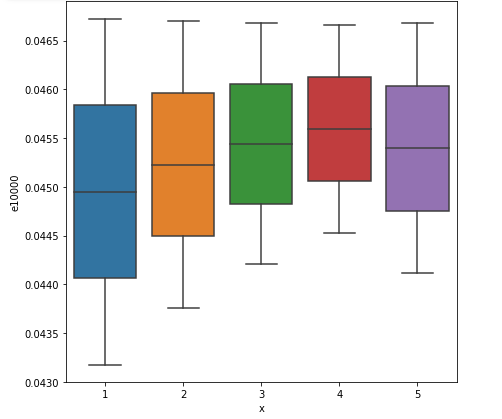
\includegraphics[width=\linewidth]{e10000.png}
		\caption{Tamaño de la muestra 10000.}
		\label{1}
	\end{subfigure}
		\begin{subfigure}[b]{0.45\linewidth}
		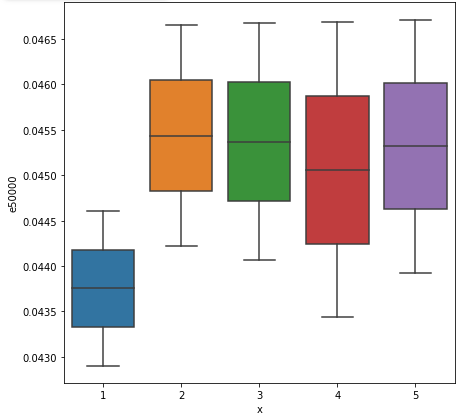
\includegraphics[width=\linewidth]{e50000.png}
		\caption{Tamaño de la muestra 50000.}
		\label{2}
	\end{subfigure}
		\begin{subfigure}[b]{0.45\linewidth}
			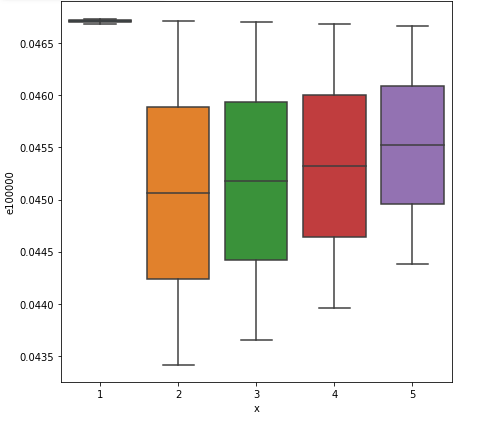
\includegraphics[width=\linewidth]{e100000.png}
			\caption{Tamaño de la muestra 100000.}
			\label{3}
	\end{subfigure}
		\begin{subfigure}[b]{0.45\linewidth}
				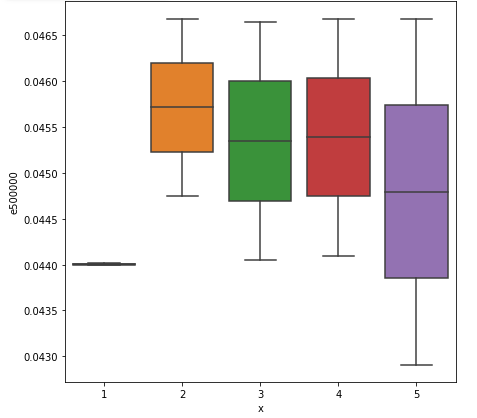
\includegraphics[width=\linewidth]{e500000.png}
				\caption{Tamaño de la muestra 500000.}
				\label{4}
	\end{subfigure}
		\begin{subfigure}[b]{0.45\linewidth}
			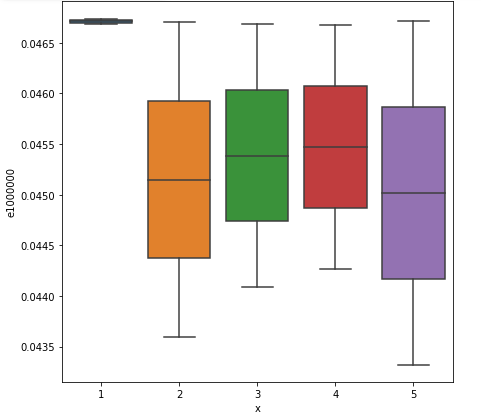
\includegraphics[width=\linewidth]{e1000000.png}
			\caption{Tamaño de la muestra 1000000.}
			\label{5}
		\end{subfigure}
	\caption{Resultados del error para los diferentes tamaños de muestras.}  		
\end{figure}



\section{Conclusiones}
Se concluye con los experimentos realizados que el aumento de los tamaños de muestras para este caso no fueron de ayuda a la hora de mejorar la solución, ya que se mantienen los valores constantes y muy alejados del valor $alpha$ que se quiere alcanzar.

\bibliography{Tarea5}
\bibliographystyle{plainnat}
\end{document} 
